\documentclass[tikz, border=1mm]{standalone}
\usepackage{amssymb}

\begin{document}
 
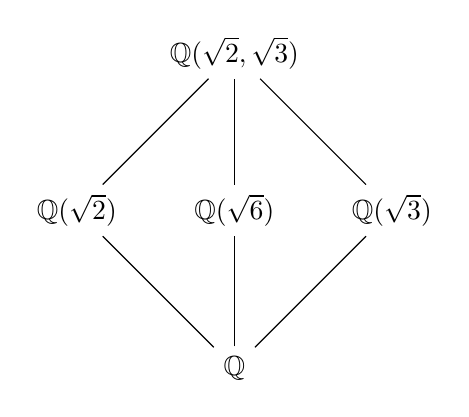
\begin{tikzpicture}[node distance = 2cm, auto]
    \node (Q) {$\mathbb{Q}$};
    \node (E) [above of=Q, left of=Q] {$\mathbb{Q}(\sqrt{2})$};
    \node (E1) [above of=Q] {$\mathbb{Q}(\sqrt{6})$};
    \node (F) [above of=Q, right of=Q] {$\mathbb{Q}(\sqrt{3})$};
    \node (K) [above of=Q, node distance = 4cm] {$\mathbb{Q}(\sqrt{2}, \sqrt{3})$};

    \draw[-] (Q) to node {} (E);
    \draw[-] (Q) to node {} (F);
    \draw[-] (E) to node {} (K);
    \draw[-] (F) to node {} (K);
    \draw[-] (Q) to node {} (E1);
    \draw[-] (E1) to node {} (K);

\end{tikzpicture}

\end{document}